\documentclass[12pt, a4paper]{book}
\usepackage[utf8]{inputenc}
\usepackage{fullpage}
\usepackage{amsmath}
\usepackage{amssymb}
\usepackage{graphicx}
\usepackage{mathtools}
\usepackage[comma,authoryear]{natbib}
\usepackage{listings}
\usepackage{color}
\usepackage{wrapfig}

\definecolor{dkgreen}{rgb}{0,0.6,0}
\definecolor{gray}{rgb}{0.5,0.5,0.5}
\definecolor{mauve}{rgb}{0.58,0,0.82}

\lstset{frame=tb,
  language=R,
  aboveskip=3mm,
  belowskip=3mm,
  showstringspaces=false,
  columns=flexible,
  basicstyle={\small\ttfamily},
  numbers=none,
  numberstyle=\tiny\color{gray},
  keywordstyle=\color{blue},
  commentstyle=\color{dkgreen},
  stringstyle=\color{mauve},
  breaklines=true,
  breakatwhitespace=true,
  tabsize=3
}
\linespread{1.3}
\graphicspath{{./}}
\title{Modeling and Forecasting US Airline Flight Delays\\2020 TAMIDS Data Science Competition}
\author{Big Data Energy\\Johnathan Lo \& Isaac Ke\\Advisor: Dr. Huiyan Sang}
\date{April 8, 2020}

\newcommand{\R}{\mathbb{R}}
\newcommand{\Z}{\mathbb{Z}}
\newcommand{\Lagr}{\mathcal{L}}
\newcommand\tab[1][1cm]{\hspace*{#1}}

\begin{document}
\maketitle
\tableofcontents
\chapter{Introduction}
\tab Reliable transportation supports a strong economy by facilitating the rapid and timely exchange of goods and services and bolstering tourism revenue. In the United States in 2018, the transportation industry accounted for \$648 billion per year, which was 3.16\% of the GDP [cite]. Worldwide, the aviation industry contributes \$2.7 trillion (3.6\%) of the world's GDP. In fact, it is projected that global air transporation will support \$5.7 trillion of the global economy [cite]. A key metric for evaluating the efficiency of airline industry production is flight delay time. In 2018, flight delays led to an economic loss of 31.2 billion dollars[cite]. For individual companies, delays can influence consumer choice, and for the industry itself, unmitigated delays can impel consumers to switch to substitute goods, such as automotive or rail-based transport. \\
\tab Therefore, a major goal of this project is to analyze flight delays and diagnose areas for improvement. We intend to create models using the provided dataset as well as publicly available data that can accurately predict future delays. In doing so, we can hopefully uncover significant and controllable covariates that can help guide airline companies to reduce flight delays. 

\chapter{Executive Summary}
	\section{Problem and Approach}
	\section{Data Preprocessing}
	\section{Exploratory Analysis}
	\section{Model Formulation}
	\section{Model Selection}
	\section{Applications and Conclusions}
	
\chapter{Motivation, Data Description, and Software}
	\section{Motivation}
	\tab As stated in the introduction, flight delays can have a wide-ranging effect on the economy. Most airline companies have already done everything in their power to mitigate and reduce delays. We are interested in finding whether delays can be further alleviated, and whether those variables can be controlled by airline companies. To the extent that some delays are unavoidable or difficult to predict, we are also interested in devising methods to minimize the impact of those delays, whether by reducing the number of passengers affected, offering alternate routes to affected passengers, or discounting tickets. Overall, for the benefit of airline companies, consumers, and society-at-large, we should minimize flight delays, or the impact thereof. 
	\section{Data Collection}
	\tab Our data was provided as .csv files by the competition organizers. The primary dataset was composed of roughly 11 million observations of 50 variables. Each observation was a distinct flight that occurred between 1/1/2018 and 6/30/2019, and the 50 covariates included origin, destination, quarter, arrival delay, departure delay, distance, and many more variables pertaining to each flight. Auxiliary datasets included information on flight routes, airports, and market share. \\
	\tab In addition to these data, we also sought out additional data to enhance our analysis. We obtained geographic coordinates for each airport from \textit{openflights.org} and historical weather data from the NOAA databases through the NCDC API [cite]. The geographic coordinates are given in decimal format, and our weather data describes meteorological events near the origin and destination of each flight. Importantly, data \textit{along} the flight path was not obtained, due to time constraints and complexity. A full list of covariates along with brief descriptions can be found in \underline{Supplementary Table 1}. 
	\section{Software}
	\tab All analyses were performed in R v3.6.3 using the RStudio IDE [cite]. Packages used include, but are not limited to, \textit{ggplot2}, \textit{ggmap}, \textit{dplyr}, \textit{caret}, \textit{rnoaa}, and \textit{tseries}. Individual datasets were loaded as \textit{data.frame} objects and combined using \textit{merge} along with various \textit{dplyr} commands . In addition, Microsoft Power BI was utilized in order to tidy the data and perform computationally-intensive data rearranging. The final dataset can be found as a .csv file in \underline{Supplementary Data 1}.
	
\chapter{Exploratory Data Analysis}

	\section{Data Wrangling}
	
	\tab Our dataset was drawn from four different main sources - flight delays and airfare data, geographic coordinates from \textit{openflights.org}, and weather data from NOAA. Flight delays and geographic coordinates were combined by merging on both common origin and destination names. The resulting data frame was then combined with fare/market data by common routes, year, and quarter. Adding weather data was more challenging in that the observations related information collected by weather stations, and not the airports themselves. Thus, weather station coordinates were cross referenced with airport coordinates to find the closest active weather station to each airport. Due to this constraint, 10 airports, corresponding to 99,980 observations (a negligable amount given the overall size of our data), were dropped due to the lack of NOAA weather stations nearby. Weather data was then merged with the rest of the data on common dates and airports, with separate variables for weather at origin and weather at destination. The final dataset containing all four sets of information is what will be referenced in this paper hereafter. Small tweaks to these data were made on a model-to-model basis, depending on the type of unique problem selected-whether it be classification or regression, for example. \\
	
	\tab The data contained a number of variables with numerical values but that could be interpreted either as quantitative or categorical variables. Using substantive knowledge, a number of numeric variables were converted to factors, including day of week, month, quarter, and route number. Additionally, our data contained many missing values. Where applicable, for categorical variables, these values were replaced by adding an additional factor level \textit{Unk}. For quantitative variables, missing values were replaced with either 0, or observations were removed, based on substantive knowledge of the variable characteristics. Finally, we discovered that the flight delay dataset somewhat bewilderingly assigned canceled flights a delay time of 0. Canceled flights were removed from the dataset and analyzed separately. Thoughout this report, we further to flight delays as specifically arrival delays as opposed to departure delays. In all, the final dataset consisted of 10,614,150 observations of 100 variables. 
	
	\section{Distribution of Flight Delays}
	
	\tab A histogram of all arrival delays is shown in \underline{Fig 1}. Clearly, the data is strongly right-skewed. To correct the skewness, a cube-root transformation was performed, but subsequent Shapiro-Wilk test provided strong evidence against normality for this transformation, so it was abandoned. To heuristically assess dependence between covariates and response, we examined various conditional distributions.\\
	\begin{wrapfigure}{l}{0.45\textwidth}
	\centering
	 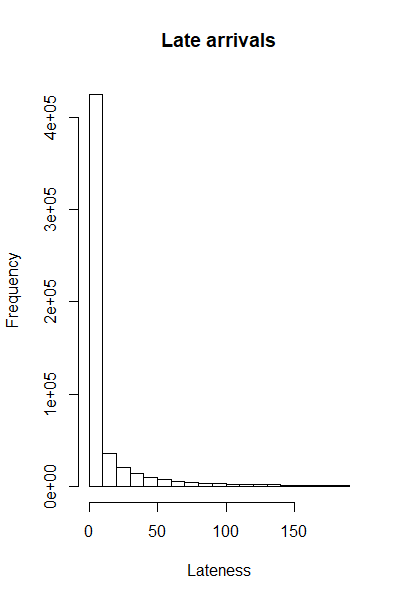
\includegraphics[width = .45 \textwidth]{../figures/LateArrivalsHistogram}
	 \caption{Fig 1 - Histogram of arrival time for all observations in the dataset}
	 \end{wrapfigure}
	 
		\subsection{Geographic Distribution of Flight Delays}
		
			\tab The distribution of flight delays across the geographic United States is shown in \underline{Fig 2}. As we can see, XXXXX XXXXX XXXXX XXXXX XXXXX XXXXX XXXXX XXXXX XXXXX XXXXX XXXXX XXXXX XXXXX XXXXX XXXXX, XXXXX XXXXX XXXXX XXXXX XXXXX XXXXX XXXXX XXXXX XXXXX XXXXX XXXXX XXXXX XXXXX XXXXX XXXXX. XXXXX XXXXX XXXXX XXXXX XXXXX XXXXX XXXXX XXXXX XXXXX XXXXX XXXXX XXXXX XXXXX XXXXX XXXXX. XXXXX XXXXX XXXXX XXXXX XXXXX XXXXX XXXXX XXXXX XXXXX XXXXX XXXXX XXXXX XXXXX XXXXX XXXXX.\\
			\begin{wrapfigure}{r}{0.45\textwidth}
			\centering
	 		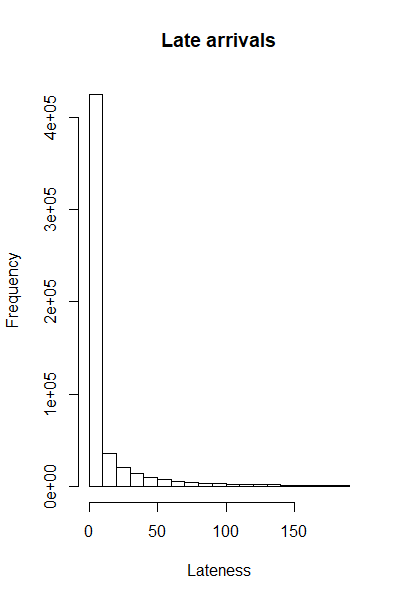
\includegraphics[width = .45 \textwidth]{../figures/LateArrivalsHistogram}
	 		\caption{Fig 2 - Figures showing the geographic distribution of flight delays by delay length and airport usage}
	 		\end{wrapfigure}
	 		
		\subsection{Temporal Distribution of Flight Delays}
		
			\tab In \underline{Fig 3}, we demonstrate the distribution of flight delays by time of day, day of week, month, and quarter.  As we can see, XXXXX XXXXX XXXXX XXXXX XXXXX XXXXX XXXXX XXXXX XXXXX XXXXX XXXXX XXXXX XXXXX XXXXX XXXXX, XXXXX XXXXX XXXXX XXXXX XXXXX XXXXX XXXXX XXXXX XXXXX XXXXX XXXXX XXXXX XXXXX XXXXX XXXXX. XXXXX XXXXX XXXXX XXXXX XXXXX XXXXX XXXXX XXXXX XXXXX XXXXX XXXXX XXXXX XXXXX XXXXX XXXXX. XXXXX XXXXX XXXXX XXXXX XXXXX XXXXX XXXXX XXXXX XXXXX XXXXX XXXXX XXXXX XXXXX XXXXX XXXXX.
			\begin{wrapfigure}{l}{0.45\textwidth}
			\centering
	 		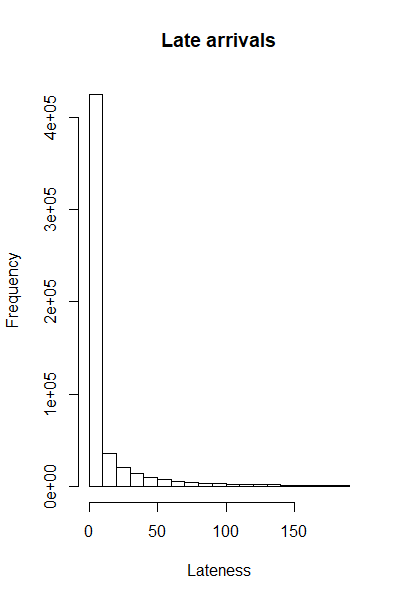
\includegraphics[width = .45 \textwidth]{../figures/LateArrivalsHistogram}
	 		\caption{Fig 3 - Histograms of ARR DELAY by time of day, day of week, month, and quarter}
	 		\end{wrapfigure}
	 		
		\subsection{Weather-based Distribution of Flight Delays}
		
			\tab Our weather data provided us primarily with data on precipitation and temperature. Other events, such as heavy fog and ice, were observed, but sparse. We show scatterplots of flight delays by precipitation and temperature in \underline{Fig 4}. In \underline{Fig 5}, histograms of flight delays for some unusual weather events are given. XXXXX XXXXX XXXXX XXXXX XXXXX XXXXX XXXXX XXXXX XXXXX XXXXX XXXXX XXXXX XXXXX XXXXX XXXXX, XXXXX XXXXX XXXXX XXXXX XXXXX XXXXX XXXXX XXXXX XXXXX XXXXX XXXXX XXXXX XXXXX XXXXX XXXXX. XXXXX XXXXX XXXXX XXXXX XXXXX XXXXX XXXXX XXXXX XXXXX XXXXX XXXXX XXXXX XXXXX XXXXX XXXXX. XXXXX XXXXX XXXXX XXXXX XXXXX XXXXX XXXXX XXXXX XXXXX XXXXX XXXXX XXXXX XXXXX XXXXX XXXXX.
			\begin{figure}[h]
	 		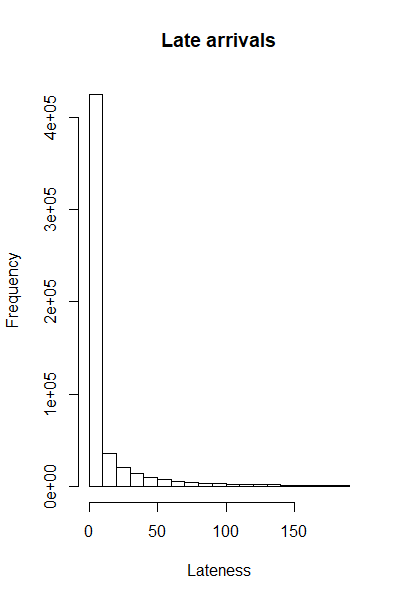
\includegraphics[width = .75 \textwidth]{../figures/LateArrivalsHistogram}
	 		\caption{Fig 4 - scatterplots of ARR DELAY by precipitation and temperature}
	 		\end{figure}
	 		\begin{figure}[h]
	 		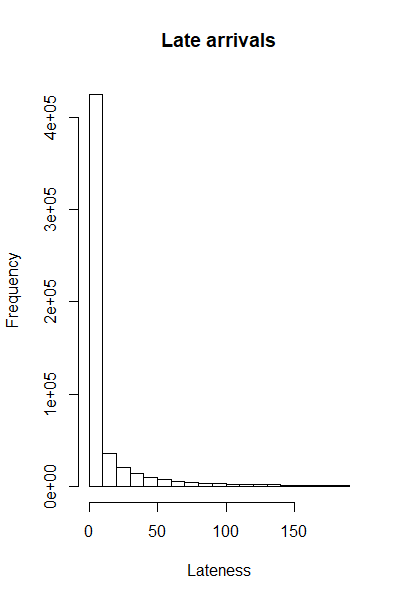
\includegraphics[width = .75 \textwidth]{../figures/LateArrivalsHistogram}
	 		\caption{Fig 5 - histograms of ARR DELAY for each unusual weather event}
	 		\end{figure}
		\subsection{Carrier-based Distribution of Flight Delays}
			
			\tab For each of the 19 carriers, flight delays was plotted. Histograms for each are given in \underline{Fig 6}. We also hypothesized that there might also be differences in flight delays between different carriers. A one-way ANOVA was conducted, and p-values corrected using Tukey's HSD, shown in \underline{Fig 7}.
			\begin{figure}[h]
	 		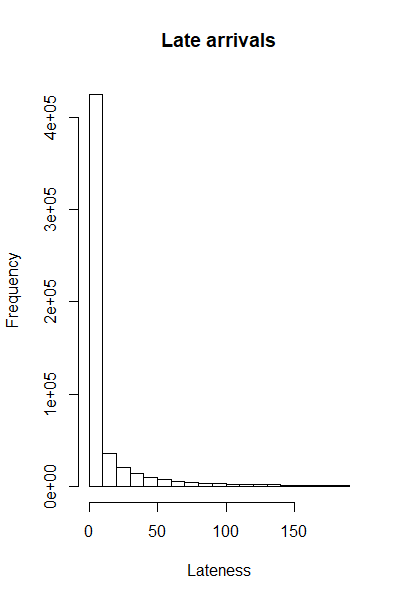
\includegraphics[width = 1 \textwidth]{../figures/LateArrivalsHistogram}
	 		\caption{Fig 6 - Histograms for the airlines}
	 		\end{figure}
	 		\begin{figure}[h]
	 		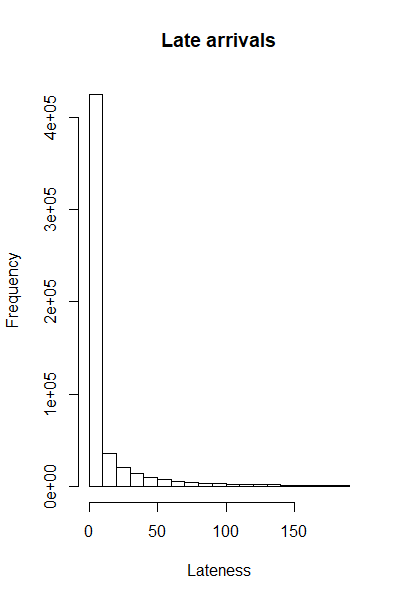
\includegraphics[width = 1 \textwidth]{../figures/LateArrivalsHistogram}
	 		\caption{Fig 7 - airline ANOVA}
	 		\end{figure}

		\subsection{Airport-based Distribution of Flight Delays}
			
			\tab We were also interesting in detecting if individual airports showed differences in flight delays, shown in \underline{Fig 8}. 
			\begin{figure}[h]
	 		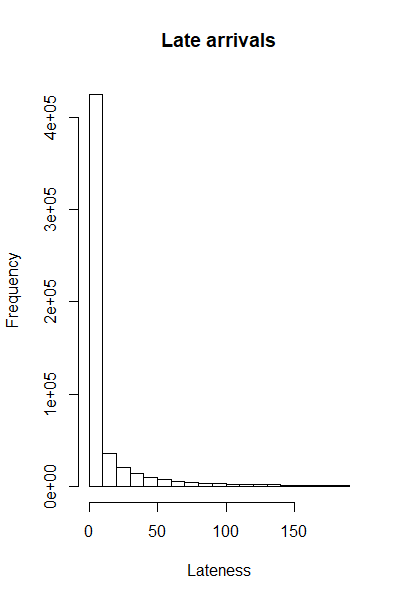
\includegraphics[width = 1 \textwidth]{../figures/LateArrivalsHistogram}
	 		\caption{Fig 8 - Airport histograms}
	 		\end{figure}
	 		
<<<<<<< HEAD
\chapter{Model formulation}
	\section{Constructing a parametric distribution for delays}
	 \tab We were interested in deducing the marginal distribution of arrival times from the data. Although it would have been relatively facile to estimate a valid empirical distribution, we decided that a parametric distribution would be more useful and intuitive. By establishing a set of parameters, further work could be directed towards estimating parameters under certain combinations of covariate values. With mostly categorical data, it then becomes feasible to estimate parameters for certain combinations of interesting variables. Parameterization also allows the density functions of the distribution to be readily expressed analytically.\\
	\tab As seen in \underline{Fig 1}, the marginal distribution is strongly right skewed, and thus our first plan of action was to attempt a transformation to correct the skewness. A number of transformations were considered. With negative values in the data, log or square root transformations could only be applied by first shifting the data to be strictly positive. One way to do this would be to simply add the smallest (most negative) number to each of our delay times; however, it was decided that this approach rendered our results somewhat uninterpretable. Consider, for example, a new observation where the flight arrived earlier (with a flight delay time more negative) than any other flight in the dataset. Such an observation would not be supported in a distribution of log-transformed values. We also briefly considered cube root transformation, but as seen in \underline{Fig 9}, it does not result in normality or resemblance to any familiar parametric distribution. In lieu of transforming the data, we considered several well-known skewed distributions, but none of them fit well or appeared sensible.
			\begin{wrapfigure}{l}{0.35\textwidth}
			\centering
	 		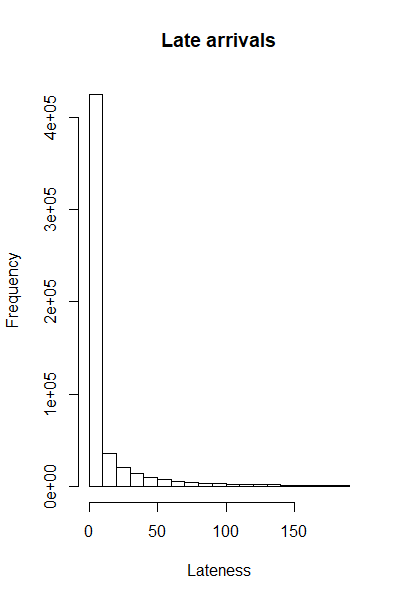
\includegraphics[width = .35 \textwidth]{../figures/LateArrivalsHistogram}
	 		\caption{Fig 9 - density plot of cube root transformation vs normal distribution with same mean and variance}
	 		\end{wrapfigure}
	\tab Thus, we instead looked to construct a mixture distribution. The primary issue that we had been confronted with this far was finding a distribution that appeared to have sensible parameterizations.  Our search was rooted in the premise that not all delays are created equal;  we suspected that the majority of delays are "run-of-the-mill" events that do not result from any extraordinary circumstances in particular, while a minority of delays have true, substantial causes. This is similar to the rationale for a zero-inflated Poisson in manufacturing processes, in that most machines are in good working order and do not produce any products with defects, but some machines with defects will produce defective products by a Poisson distribution. As such, we decided upon a mixture of the form \begin{center}$$Y = UV + (1-U)T$$\end{center} with $U\sim Ber(p)$, $V\sim N(\mu,\sigma^2)$, and $T\sim exp(\lambda)$. In this model, $U$ describes whether or not a delay with "true, substantial causes" occurs, $V$ describes the distribution of arrival times when no extenuating circumstances occur, and $T$ describes arrival times under defined circumstances that result in lateness. Using MLE, we were able to generate estimates of the parameters for the marginal data, as shown in \underline{Fig 10}.
			\begin{wrapfigure}{l}{0.45\textwidth}
			\centering
	 		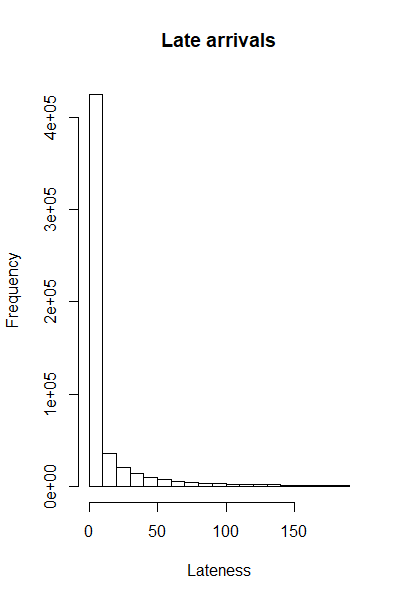
\includegraphics[width = .45 \textwidth]{../figures/LateArrivalsHistogram}
	 		\caption{Fig 10 - Histogram of samples from distribution given by MLE, and histogram of values from data (fig 9)}
	 		\end{wrapfigure}
	\tab To validate this distribution, a QQ plot was made of the observed arrival times against the mixture distribution under the parameter estimates from the MLE (\underline{Fig. 11}). From this plot, it can be observed that our mixture distribution is in fact able to describe the observed values of arrival time quite accurately. Note that the arrival times are given as discrete values (as minutes), hence the "jumps" from percentile to percentile. It is important to note here, however, that our distribution does fail to describe data points in the extreme upper range of observations. 
			\begin{wrapfigure}{r}{0.45\textwidth}
			\centering
	 		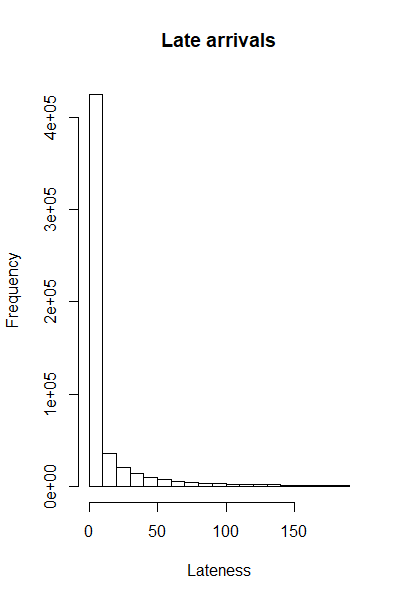
\includegraphics[width = .45 \textwidth]{../figures/LateArrivalsHistogram}
	 		\caption{Fig 11  - QQ plot of of data vs theoretical distribution}
	 		\end{wrapfigure}
	\tab An additional approach to validating this distribution would be through conditional density estimation.
\chapter{Model selection}
=======
\chapter{Model Formulation}
\chapter{Model Selection}
>>>>>>> b23702e2b03bee766bafd1c387ec066737496501
\chapter{Forecasting Flight Delays for 2019 Q3}
\chapter{Business Recommendations}
\chapter{Closing Thoughts}
\chapter{Appendix}
	\section{References}
	\section{Additional Figures, Tables, Code, and Data}
\pagebreak

\bibliographystyle{natdin}
\nocite{*}
\bibliography{sources}
\end{document}